\usetikzlibrary{arrows.meta,calc}

\begin{frame}[fragile,label=throughAndWindow]{throughput and window size}
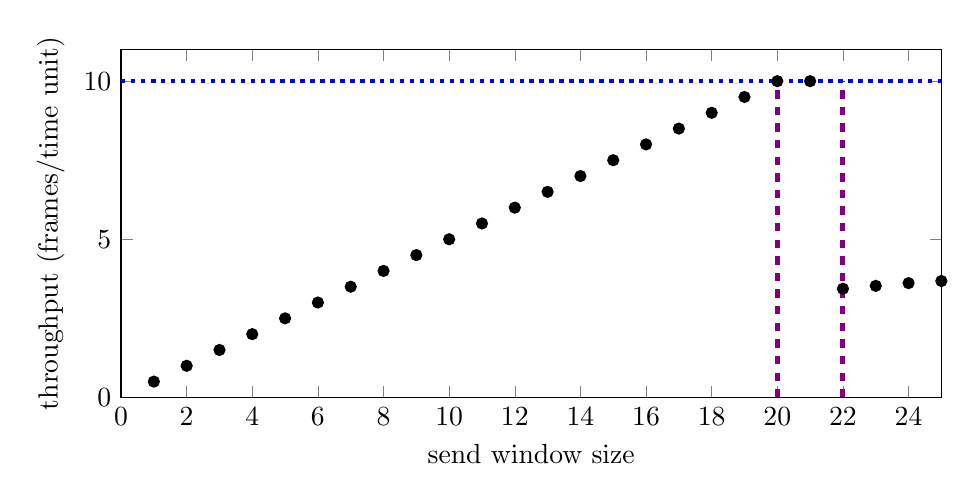
\begin{tikzpicture}
\begin{axis}[width=12cm,height=6cm,
    xlabel=send window size,
    ylabel=throughput (frames/time unit),
    xmin=0,xmax=25,ymin=0]
\addplot[only marks] coordinates {
(1, 0.5000025000125)
(2, 1.0000090000810007)
(3, 1.4999925000374998)
(4, 2.0000280003920055)
(5, 2.500037500562508)
(6, 3.000003000003)
(7, 3.5000035000035)
(8, 4.000048000576006)
(9, 4.499842505512307)
(10, 5.000025000125)
(11, 5.499975250111374)
(12, 5.99977200866367)
(13, 6.499710762871052)
(14, 6.999811005102861)
(15, 7.4996812635462975)
(16, 7.999680012799485)
(17, 8.499426288725509)
(18, 8.999361045365776)
(19, 9.499202067026369)
(20, 9.999100080971061)
(21, 9.999100080973866)
(22, 3.435635094325549)
(23, 3.5274986154570636)
(24, 3.613708966335035)
(25, 3.6808686850100703)
(26, 3.753260645186032)
(27, 3.8487443471573166)
(28, 3.925956461143474)
};
\addplot[blue,dotted,ultra thick,domain=0:25] {10};
    \draw[violet,dashed,ultra thick] (axis cs:20,0) -- (axis cs:20, 10)
     coordinate (empty queue mark);
    \draw[violet,dashed,ultra thick] (axis cs:21.99,0) -- (axis cs:21.99, 10)
     coordinate (full queue mark);
\end{axis}
\end{tikzpicture}
\end{frame}
